%!TEX root = flock-comment-main.tex

\section*{Introduction}
In most fields, proposed methods that are 
perceived to be fundamentally novel or new garner more
attention and accolades---and have a higher chance of publication---
than methods that are clearly minor elaborations upon existing work. 
Not surprisingly, then, in articles and manuscripts, authors may 
emphasize the differences and downplay the similarities between their 
work and the published literature.   In molecular ecology, this 
tendency amongst the creators of statistical methodology can make it 
difficult for end-users to understand the relationship between 
different methods.

Of course, new methods almost always build upon pre-existing ones, and 
much is to be gained by understanding the close relationship between 
different statistical methods in use in molecular ecology today.  
Indeed, some authors downplay the similarities between their method and 
existing ones not because they wish to make their method seem more 
novel, but rather because they are genuinely unaware of the close ties 
between their work and existing methods.  Identifying the 
similarities between new and existing work should help the field 
progress more quickly by 1) reducing end-user confusion about whether 
it is necessary to analyze data with a (sometimes overwhelming) variety 
of computer programs; 2) establishing a common language upon which to 
compare different methods; and 3) providing a principled perspective 
from which to argue about the expected strengths and weaknesses of any 
method.

Methods for the unsupervised clustering of genotypes have received 
considerable attention in the molecular ecology literature.  
The best known example of this class of methods is {\sc structure} 
\citep{Pritchardetal2000}.  {\sc structure} itself can be described 
as an elaboration of earlier models used to identify the spawning 
stock of salmon \citep{Smouseetal1990}, and a variety of other 
clustering methods have been developed that are all closely related to 
{\sc structure}, for example {\sc NewHybrids} \citep{And&Tho2002}, {\sc 
BayesAss+} \citep{Wil&Ran2003}, and {\sc baps} 
\citep{Coranderetal2004}. An overview of these similarities can be 
found in \citet{Anderson2009PGAC}.

Recently, a description of the software {\sc flock} was published, 
billing the method as a ``non-Bayesian method [that] 
differs substantially from previous 
clustering algorithms'' \citep[][p.~1333]{Duc&Tur2009}. A following
paper asserts that
\begin{quote}
``{\sc flock} is very different from  other clustering 
programs. It does not sample the space of partitions through small 
random step walks as in MCMC, and it does not try to optimize some 
target function, such as HWLE\@. Briefly stated, it is not based on a 
probabilistic search algorithm. On the contrary, {\sc flock} is 
entirely deterministic'' \citep[][p.~736]{Duc&Tur2012}.
\end{quote}
These papers describe the rationale behind the {\sc flock} algorithm in
intuitive terms with analogies to the coalescence of flocks of birds
or the accretion of snow on a moving snowball, \etc.  

Here, we provide a different perspective on the {\sc flock} algorithm,
showing it to be a special, restricted case of the simulated annealing
algorithm for finding the Bayesian maximum {\em a posteriori} (MAP)
estimate from a marginalized form of the {\sc structure} model with no
admixture and non-correlated allele frequencies. 

\section*{Comparison of methods}
We start with a succinct mathematical description of the {\sc structure}
algorithm, then describe the {\sc flock} algorithm, and finally explain
the close relationship between the two.


\subsection*{{\sc structure}}
In the {\sc structure} model with no admixture, the unknown ``subpopulation'' that the 
$i\thh$ individual ($i=1,\ldots,N)$ belongs to is denoted by $Z_i \in \{1,\ldots,K\}$, where $K$ is the 
number of subpopulations (or clusters, as they are often referred to).  
In a diploid individual from cluster $k$, the 
allelic types of the two gene copies at the $\ell\thh$ locus are assumed
to be drawn independently from the vector of allele frequencies at
locus $\ell$,  $\theta_{k\ell}=(\theta_{k\ell 1},\ldots,\theta_{k\ell A_\ell})$, where $A_\ell$ 
denotes the number of alleles observed in the data set at locus $\ell$.
Hence, if $Y_{ij}$ denotes a vector of length $A_\ell$ whose components denote the number
of copies of each of the $A_\ell$ alleles at locus $j$ in individual $i$, and 
$Z_i=k$, then $Y_{i\ell}$ follows the multinomial distribution of two trials with
with $A_\ell$  components and cell probabilities given by the allele frequencies: 
\begin{equation}
(Y_{i\ell}~|~Z_i=k) \sim \mathrm{Mult}_{A_\ell}(2, \theta_{k\ell}).
\end{equation}
In the model without physical linkage, the genotypes at the loci are assumed to
be independent of one another, so the probability of the genotype data at
all $L$ loci---$Y_i=(Y_{i1},\ldots,Y_{iL})$---is simply a product of multinomial probabilities.
In the uncorrelated allele frequencies model, the prior on each $\theta_{k\ell}$ is a
Dirichlet distribution with parameters $(\lambda_{k\ell1},\ldots,\lambda_{k\ell A_\ell})$,
which are usually set to a value like $1/A_\ell$.  

Inference in the model proceeds by sampling from the joint posterior of the 
$Z_i$'s and $\theta = (\theta_1,\ldots,\theta_K)$ using Gibbs sampling.  That is,
at iteration $t$:
\begin{enumerate}
\item each $Z^{(t)}_i$ is updated to $Z^{(t+1)}_i$ by sampling a value from 
the full conditional distribution of $Z_i$ given
$Y_i$ and $\theta^{(t)}$ (the current estimate of the allele frequencies).  This
distribution is found using Bayes' theorem. In {\sc structure}'s formulation, the 
prior probability that $Z_i=k$ is $1/K$ for all $k=1,\ldots, K$.     
\item $\theta^{(t)}$ is updated from its full conditional distribution.  For each cluster
$k$, and locus $\ell$ the full conditional for $\theta_{k\ell}$ is independently a 
Dirichlet distribution with parameters $\lambda_{k\ell j} + \#(k,\ell,j)$, for $j=1,\ldots, A_\ell$,
where $\#(k,\ell,j)$ is the number of alleles of type $j$ at locus $\ell$ observed in 
individuals whose $Z^{(t+1)}_i = k$.   
\end{enumerate}

It will be useful for our comparison with {\sc flock} to point out that another way 
of pursuing inference in this model would be to first integrate out the 
Dirichlet priors on the allele frequencies and then sample from the posterior
for the $Z_i$'s by Gibbs sampling.  When $\theta$ is integrated out, the genotypes 
of the individuals are no longer conditionally independent (they were originally
independent {\em conditional} on $\theta$ and the $Z_i$'s), so the calculation of 
the full conditional distribution of $Z_i$ is now somewhat more involved: the full 
conditional distribution of $Y_{i\ell}$ given $Z_i=k$, and $Z_{(-i)}$ and $Y_{(-i)\ell}$---the
cluster memberships and genotypes, respectively,  of all the remaining individuals---is
now a Compound Dirichlet Multinomial distribution (CDM):
\begin{eqnarray}
\lefteqn{(Y_{i\ell}~|~Z_i=k,~Z_{(-i)},~Y_{(-i)\ell}) \sim} \label{eq:cdm}\\
& & \mathrm{CDM}(\lambda_{k\ell 1} + \#_{(-i)}(k,\ell,1), \ldots,
\lambda_{k\ell A_\ell} + \#_{(-i)}(k,\ell,A\ell)), \nonumber
\end{eqnarray}
where $\#_{(-i)}(k,\ell,1)$ is the number of alleles of type $j$ at locus $\ell$
found in individuals {\em other than individual $i$} that currently
belong to cluster $k$. Calculating (\ref{eq:cdm}) for each value of $Z_i=k \in \{1,\ldots,K\}$ 
and normalizing to sum to one gives the full conditional distribution for 
$Z_i$:
\begin{equation}
P(Z_i=k~|~Y_i, ~Z_{(-i)},~Y_{(-i)\ell})~~,~~k=1,\ldots,K.
\label{eq:fc}
\end{equation}
A new value of $Z_i$ would be drawn from (\ref{eq:fc}) if doing Gibbs sampling in this
version of the {\sc structure} model in which $\theta$ has been integrated out.  In fact,
this is the approach (with a slightly different prior weight on the $Z_i$'s) taken to update 
$Z_i$ in both {\sc hwler} \citep{Pel&Mas2006} and {\sc structurama} \cite{Hue&And2007} when not
proposing changes to the number of clusters.



\subsection*{{\sc flock}}
One issue I have with it is that it is described as a ``procedure'' or 
an ``algorithm,'' without an attempt to see it as a special case of 
well known inference frameworks.


\subsection*{{\sc flock} as a special case of {\sc structure}}

\section*{Results}

\subsection*{{\sc flock} analysis of coasta California steelhead} 
{\sc flock} was run four times using the default setting for all run parameters \textit{(initial partition = random, number of iterations = 20, number of runs = 50, LLOD threshold = 0)} for values of \textit{k} from 2 to 6. The stopping point of \textit{k}=6 was chosen because four consecutive runs with 0 length plateaus were produced. 
Run times were relatively short. The four groups of runs for the default settings averaged 217 minutes (30min SD) on an i7 3.40GHz processor with 8GB of RAM. While no plateaus were observed in any of the four groups for a \textit{k} greater than two, the plateau record varied greatly among each group for \textit{k}=2 (plateau sequences- Run1=3,2,5,6,3; Run2=2,2,2,4,3,2; Run3=2,3,2,4; and Run4=2,3,3,4,2,2,5,2). The plateau analysis procedure suggested by \citet{Duc&Tur2012} leads to two different conclusions for the plateau sequences observed: \textit{k}=2 is the lower bound estimate (Run1) or there is no estimate (\textit{undecided}: Runs 2-4). Despite different conclusions, the allocation of individuals for the 'best run' from each group differed by a only a single individual. When \textit{k}=2, {\sc flock} identifies a boundary in the Russian Gulch area clustering individuals into northern and southern groups (Fig. 1). 

\begin{figure}
    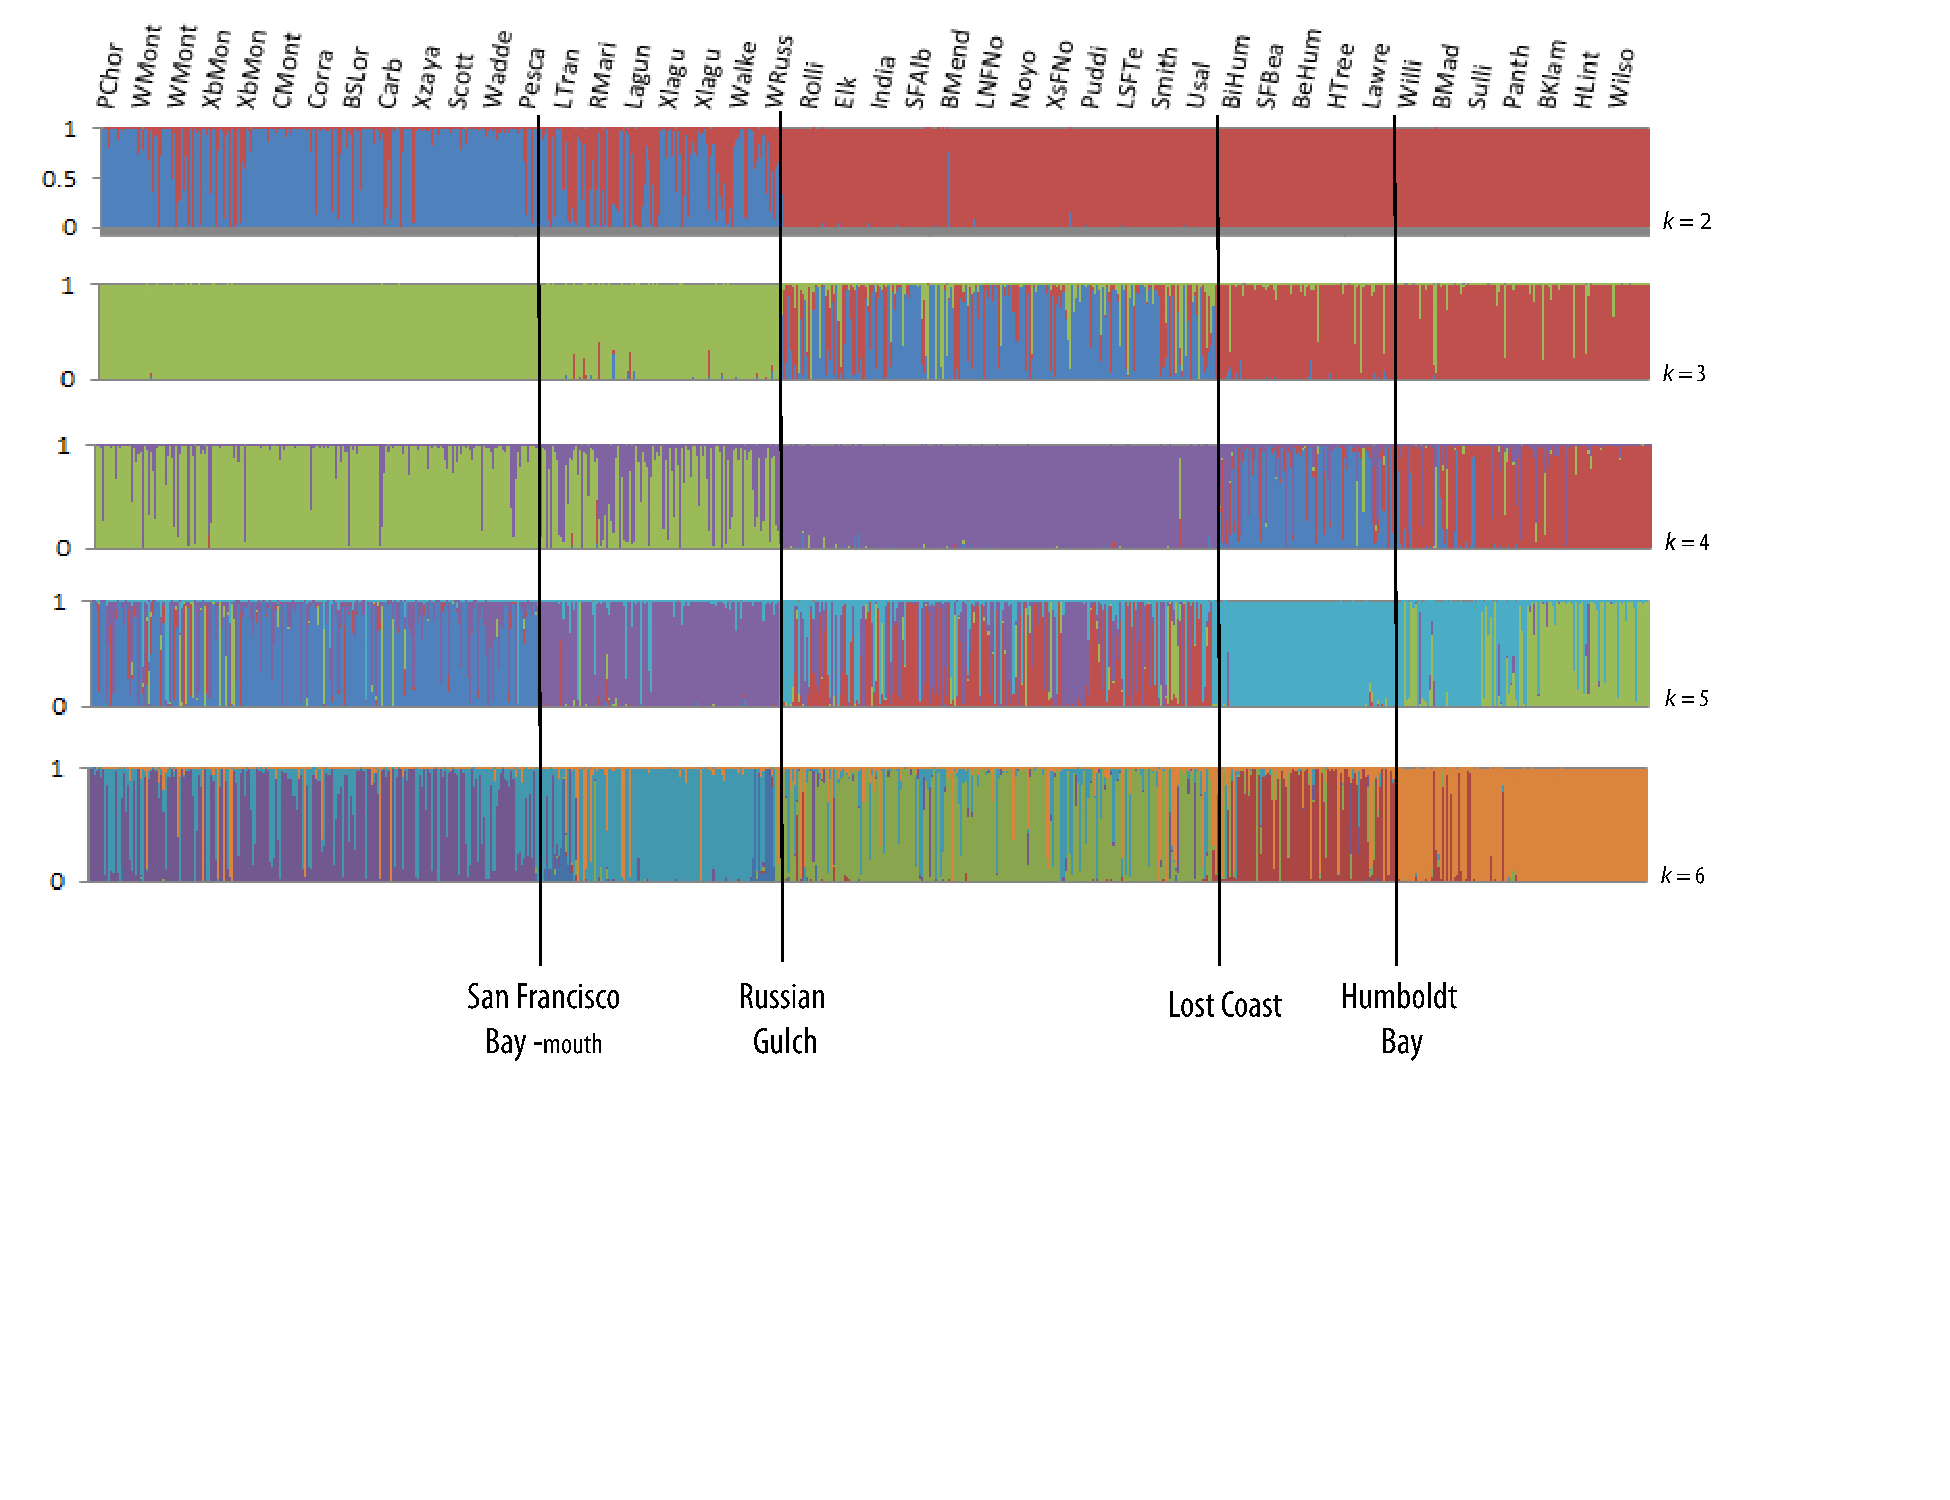
\includegraphics[width=8.0in]{FLOCK_OneSampDefault.tif}
    \caption{Assignment to reference population (from \textit{k} = 2-6) plots created in the program {\sc flock}. Each horizontal plot represents the 'best run' from a series where individuals are reallocated into \textit{k} clusters. Within each plot the normalized individual likelihood for each reference population is represented by a colored vertical bar. Major geographic boundaries that were attributed to genetic structure in \citet{Garzaetal_norcal} are indicated with black vertical lines. Results from the 'best runs' showed similar geographic differentiation to \citet{Garzaetal_norcal} analysis. The plateau analysis developed by \citet{Duc&Tur2012} indicate that either an undecided structure or that \textit{k}=2 is the lower bound estimate.}
    \label{Fig.1}
\end{figure}

With increased \textit{k} {\sc flock} continues to splits individuals approximately based on geographical boundaries identified by \citet{Garzaetal_norcal} using {\sc structure}. Once \textit{k} = 6 is reached no new regions are identified.

To investigate the ability of the arrangement of individuals within the reference populations to move around the partition space we varied the number of iterations that each run goes through to find the 'optimal' allocation of individuals. Unfortuantely only the reallocation matrix for the 'best run' is given as output. Increasing the number of iterations did not affect the overall inference of \textit{k}. It was observed that often during the last iterations individuals would alternate between reference groups during subsequent iterations. Increasing the log likelihood difference threshold for reallocation to 0.18 (there needs to be at least a 1.5 times higher likelihood to reallocate the individual) minimized this, but did not affect the inference of \textit{k} (lower bound estimate of \textit{k} = 2). 


\section*{Conclusions}
The partition space over which {\sc flock} evaluates how individuals are clustered greatly increases with both the number of individuals and the number of clusters into which they can be partitioned. The total partition space for any given k can be defined by $\sum\limits_{i=1}^k S(n,k)$ where S(n,k) is a Stirling number of the second kind. The results of {\sc flock} depend primarily on the initial partition of individuals. It is not surprising that with 2,596 individuals we could have drastically different plateau sequences with just two clusters. It is difficult to access how well the reallocation process moves the cluster of individuals within the partition space due to the fact that the reallocation matrix from only the 'best-run' is reported. 
